\small
\begin{tabular}{c|cccccccc}
$q$ & $g_0$ & $g_1$ & $g_2$ & $g_3$ & $g_4$ & $g_5$ & $g_6$ & $g_7$\\\hline
0&0&1&2&3&4&5&6&7\\
1&1&2&3&4&5&6&7&0\\
2&2&3&4&5&6&7&0&1\\
3&3&4&5&6&7&0&1&2\\
4&4&5&6&7&0&1&2&3\\
5&5&6&7&0&1&2&3&4\\
6&6&7&0&1&2&3&4&5\\
7&7&0&1&2&3&4&5&6
\end{tabular}
\caption{Illustrative normalized $K=8$ cyclic schedule for $b_0=0$ and positive orientation. Secret base and orientation permute displayed labels while preserving the property that each coded symbol visits all eight clusters once per complete cycle.}
\Description{Eight-by-eight cyclic table in which each row is shifted by one label, so every coded symbol maps to every cluster exactly once over eight sessions.}
\label{fig:cycle}
\end{figure}

\subsection{Finite-index feasibility}
For protected envelope $c$, let $d_k(c)$ denote the number of group occurrences required for label $k$ after coding and session mapping, and $a_k$ the number of available groups in label bank $k$. The session is feasible when
\begin{equation}
d_k(c)\le a_k \qquad \text{for every }k.
\end{equation}
Nominal alphabet capacity $\log_2 K$ gives coded bits per label, while this condition tests complete-message realizability under finite group availability and within-session unique-cover usage.

Two exact properties hold before experimental evaluation. First, for any fixed coded symbol $v$ and starting sequence $q_0$, the multiset $\{\pi_{q_0+t}(v):0\le t<K\}$ contains every cluster label exactly once. Second, under unique-cover usage and a preconstructed group bank, the finite-index inequality is necessary and sufficient for emitting the complete coded session: each occurrence consumes one distinct group of its mapped label, and any feasible demand vector can be assigned distinct available groups label by label.

\begin{table}[t]
\caption{Role of principal components and evidence supporting each role.}
\label{tab:roles}
\small
\begin{tabularx}{\textwidth}{p{2.5cm}Y Y}
\toprule
Component & Protocol role & Evidence/guarantee\\
\midrule
Calibration-locked projection & Define an externally fixed $K=8$ label space & Selection uses calibration attacks; holdouts remain reserved for validation\\
Complementary five-cover bank & Convert heterogeneous per-cover failures into majority decisions & Group failure signatures and 1,800/1,800 external calibration recoveries\\
RS128 & Correct residual coded-byte errors & Up to 37 corrections in calibration and 64 on holdout crop\\
Cyclic keyed Gray map & Balance coded-symbol-to-cluster assignment & Exact $K$-session algebraic balancing property\\
Signature-balanced scheduler & Preserve calibration-failure-signature mixture during keyed selection & Proportional-deficit scheduling followed by independent detector audit\\
AES-GCM + sequence/replay state & Authenticate accepted plaintext and session metadata & Standard AEAD semantics, explicit nonce discipline, stateful replay rejection\\
\bottomrule
\end{tabularx}
\end{table}

\section{Experimental Design}
\subsection{Development and external evidence}
BOSSBase 1.01 provides the development corpus for protocol design and operating-point selection. The final development lineage uses the same $K=8$, group-size-5, RS128, 30-session construction later frozen for external validation. Caltech-101 supplies the external corpus, with 9,144 readable source images. For each seed in $\{11,29,47,71,101\}$, a deterministic permutation assigns 1,500 images to descriptor training and the next 7,000 images to the cover index. These two sets are image-disjoint. Caltech images are converted uniformly to RGB before the $256\times256$ channel fit.

The frozen external operating point uses $K=8$, group size five, 128 parity bytes, and 30 authenticated sessions per partition. Ten deterministic plaintexts are generated at each of 8, 32, and 64 bytes; authenticated sequences are 0--9, 10--19, and 20--29 respectively. A public deterministic benchmark root derives partition-specific keys and nonces for reproducibility; deployment key management remains a separate operational layer.

\subsection{Calibration and holdout channel tests}
The twelve calibration transformations are those listed above. The holdout set contains eight intermediate or stronger transformations: Gaussian noise 9 and 15; blur 1.2 and 1.8; central crop 8\% and 12\%; and rotations 5 and 9 degrees. Each of 30 sessions is evaluated under every transformation for each of five partitions, yielding 1,800 calibration trials and 1,200 holdout trials. Trial success requires exact authenticated plaintext recovery, so symbol accuracy and error-correction counts remain diagnostic quantities beneath the final message-level criterion.

\subsection{Selection-detectability audit}
The detector audit reconstructs the complete 30-session selected-cover schedule for every external partition. For each partition and each of 20 repetitions, a 65/35 image-disjoint train/test split is created. The same split is used across three detector families: SRM-lite residual features with ExtraTrees, GLCM texture features with logistic regression, and a 30-head CNN audit. Reported AUCs are macro-averaged at repetition level; repeated-split intervals describe empirical variability because splits overlap and are not interpreted as independent inferential confidence intervals.

\subsection{Frozen DiffStega reproduction}
The DiffStega comparison executes the public upstream implementation at commit \texttt{73cd7cb8d102\allowbreak f4fc0f5bb168\allowbreak a71cfb948077\allowbreak d89a} on all 100 UniStega cases: 30 similar-prompt, 42 content-prompt, and 28 style-prompt cases. The execution produces 700 PNG outputs. Metric extraction is performed independently and preserves the distinct semantics of secret-image reconstruction. The evidence bundle is identified by SHA-256 \texttt{32d0e975eb19\allowbreak 7adb0d1d2f7c\allowbreak 537b04b4fab8\allowbreak 4af45a51148e\allowbreak af15872b40de\allowbreak 1f46}.

\section{Results}
\subsection{Development evidence on BOSSBase}
The frozen $K=8$ development lineage reaches 1,800/1,800 calibration recoveries across five seeds. Cover participation is near-complete, with 7,995--8,000 unique covers exercised per seed. Table~\ref{tab:boss} reports the development diagnostics retained before external evaluation.

\begin{table}[t]
\caption{BOSSBase development evidence for the frozen $K=8$ lineage.}
\label{tab:boss}
\small
\begin{tabular}{rrrrrr}
\toprule
Seed & Stable & Unique & Freq. CV & Global7 AUC & Clean15 AUC\\
\midrule
11 & 5,836 & 8,000 & 0.262 & 0.5187 & 0.5231\\
29 & 5,193 & 7,995 & 0.253 & 0.5127 & 0.5182\\
47 & 4,926 & 8,000 & 0.257 & 0.5102 & 0.5184\\
71 & 5,369 & 8,000 & 0.257 & 0.5177 & 0.5171\\
101 & 5,135 & 8,000 & 0.252 & 0.5100 & 0.5150\\
\midrule
Mean & 5,292 & 7,999 & 0.256 & 0.5139 & 0.5184\\
\bottomrule
\end{tabular}
\end{table}

\begin{figure}[t]
\centering
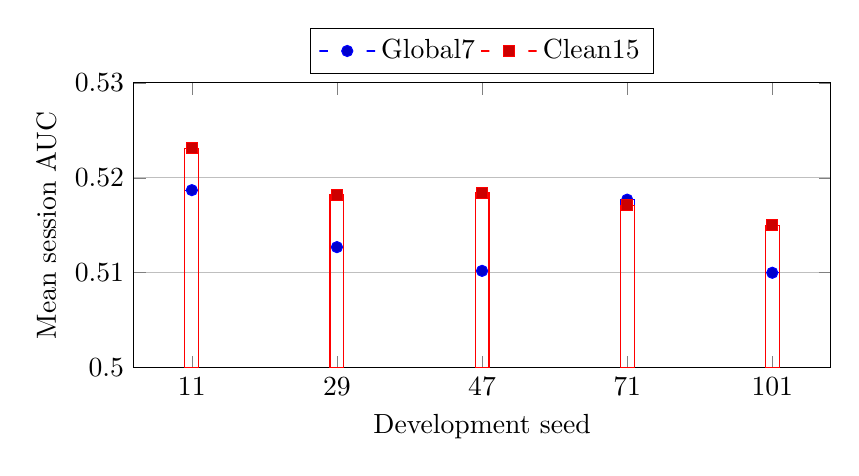
\begin{tikzpicture}
\begin{axis}[width=.86\textwidth,height=5.2cm,ymin=.5,ymax=.53,xtick={1,2,3,4,5},xticklabels={11,29,47,71,101},xlabel={Development seed},ylabel={Mean session AUC},legend style={at={(0.5,1.03)},anchor=south,legend columns=2},ymajorgrids=true]
\addplot+[ybar,bar width=5pt] coordinates {(1,.5187)(2,.5127)(3,.5102)(4,.5177)(5,.5100)};
\addplot+[ybar,bar width=5pt] coordinates {(1,.5231)(2,.5182)(3,.5184)(4,.5171)(5,.5150)};
\legend{Global7,Clean15}
\end{axis}
\end{tikzpicture}
\caption{BOSSBase development-stage selection diagnostics for the frozen $K=8$ lineage. Both diagnostic families remain close to the 0.5 chance reference across seeds.}
\Description{Grouped bar chart of Global7 and Clean15 development AUC values for seeds 11, 29, 47, 71, and 101; all values are near 0.5.}
\label{fig:bossauc}
\end{figure}
